\documentclass[10pt,a4paper]{report}
\usepackage[T1]{fontenc}
\usepackage[utf8]{inputenc}
\usepackage[colorlinks]{hyperref}
\usepackage{tabularx,xltabular}
\usepackage{imakeidx}
%\usepackage[acronym]{glossaries}
\usepackage[acronym,nopostdot,toc]{glossaries-extra}
%\usepackage{glossaries}
\usepackage{graphicx}
\usepackage{textcomp,upquote,listings}
\usepackage{mathtools}
%\usepackage{amsmath}


%%\newglossary*{general}{General}
%%\newglossary*{web}{Web}
%%\newglossary*{web}{Web}
%%\newglossary*{linux}{Linux}
%%\newglossary*{windows}{Windows}
%% Generate the glossary
%%\makeglossaries

%%\loadglsentries{glossary-win}
%%\loadglsentries{glossary-general}

%\newcommand{\indexgls}[1]{\expandafter\index\expandafter[\expandafter m\expandafter]\expandafter{\glsentrytext{#1}@\gls{#1}}}
%\makeindex[program=makeindex,options=-s ,columns=3,intoc=true]
\makeindex

\setcounter{tocdepth}{3}
\setcounter{secnumdepth}{3}

\title{My Red Team Bible}

\begin{document}
\lstset{language=Python,upquote=true}
\maketitle
\part{table of contents}
\tableofcontents
\clearpage
\part{Knowledge}
\chapter{Portable Executable }
\label{knowledge:pe}
\section{Introduction}


Executable files follow a standardized structure called the {\bf Common Object File Format (COFF)}.

\href{https://learn.microsoft.com/en-us/windows/win32/debug/pe-format}{Portable Executable} Files are a COFF formatted executable encapsulating formats such as Executable (.exe, .cpl, .sys, etc), object code and DLLs. 

The PE file format contains integral information required by the Windows OS to efficiently load and execute the file.  

\section{Structure}
\subsection{Introduction}

\href{https://learn.microsoft.com/en-us/windows/win32/debug/pe-format}{PE Format} official documentation describe default values 

\href{https://www.openrce.org/reference_library/files/reference/PE%20Format.pdf}{Open RCE - PE Format}

\begin{figure}[!ht]
    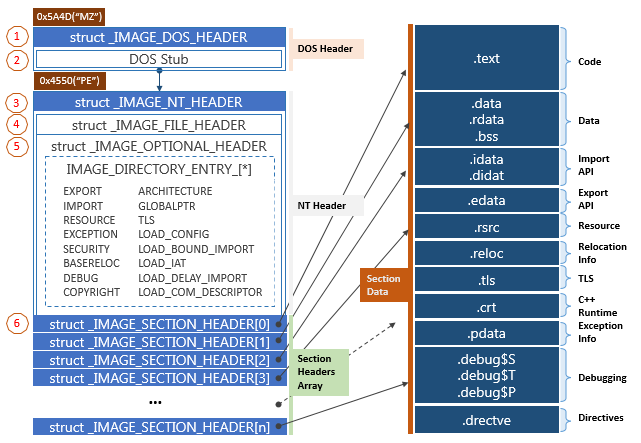
\includegraphics[width=\linewidth]{knowledge/pe/images/Gen_DD_Win_PE_Format.png}
    \caption{PE overview}
    \label{fig:pe_overview}
\end{figure}

\begin{figure}[!ht]
    \includegraphics[width=\linewidth]{knowledge/pe/images/pe-format.pdf}
    \caption{PE Details}
    \label{fig:pe_details}
\end{figure}

All structures are defined in \href{https://learn.microsoft.com/fr-fr/windows/win32/api/winnt/}{winnt.h}

\subsection{Relative Virtual Address}
An RVA specifies the offset of an element (like a function, data structure, or section) from the base address where the PE file is loaded into memory.

When a PE file is loaded into memory, the operating system assigns it a {\bf base address}. This is the starting point in virtual memory where the entire image of the PE file is mapped.

Mathematically: \verb+RVA=Virtual Address - Base Address+

Absolute Virtual Address is the \verb-RVA + Base Address-

RVAs are heavily used in the PE file's import and export tables to specify the locations of functions and data. For example, the addresses of imported functions are given as RVAs, which are resolved to actual virtual addresses at runtime.

RVAs are crucial for relocating a PE file when it cannot be loaded at its preferred base address. The loader adjusts all RVAs accordingly.

the PE file sections are aligned differently in memory compared to how they are laid out on disk, the RVA does not directly correspond to an offset in the file. 

To convert an RVA to a file offset (or vice versa), you need to:
\begin{itemize}
    \item Identify the section in which the RVA falls.
    \item Use the section's information (like \verb+PointerToRawData+ and \verb+VirtualAddress+) to compute the corresponding file offset.
\end{itemize}


\subsection{DOS}

\subsubsection{DOS Header}
The DOS header (also called the MS-DOS header) is a 64-byte-long structure that exists at the start of the PE file.

It’s there because of backward compatibility reasons. 

This header makes the file an MS-DOS executable, so when it’s loaded on MS-DOS the DOS stub gets executed instead of the actual program.
Without this header, if you attempt to load the executable on MS-DOS it will not be loaded and will just produce a generic error.

\begin{verbatim}
typedef struct _IMAGE_DOS_HEADER {      // DOS .EXE header
  WORD   e_magic;                     // Magic number
  WORD   e_cblp;                      // Bytes on last page of file
  WORD   e_cp;                        // Pages in file
  WORD   e_crlc;                      // Relocations
  WORD   e_cparhdr;                   // Size of header in paragraphs
  WORD   e_minalloc;                  // Minimum extra paragraphs needed
  WORD   e_maxalloc;                  // Maximum extra paragraphs needed
  WORD   e_ss;                        // Initial (relative) SS value
  WORD   e_sp;                        // Initial SP value
  WORD   e_csum;                      // Checksum
  WORD   e_ip;                        // Initial IP value
  WORD   e_cs;                        // Initial (relative) CS value
  WORD   e_lfarlc;                    // File address of relocation table
  WORD   e_ovno;                      // Overlay number
  WORD   e_res[4];                    // Reserved words
  WORD   e_oemid;                     // OEM identifier (for e_oeminfo)
  WORD   e_oeminfo;                   // OEM information; e_oemid specific
  WORD   e_res2[10];                  // Reserved words
  LONG   e_lfanew;                    // File address of new exe header
} IMAGE_DOS_HEADER, *PIMAGE_DOS_HEADER;
\end{verbatim}

\begin{itemize}

    \item \verb+e_magic+: This is the first member of the DOS Header, it’s a \verb+WORD+ (2 bytes), it’s usually called the magic number. It has a fixed value of \verb+0x5A4D+ or \verb+MZ+ in ASCII, and it serves as a signature that marks the file as an MS-DOS executable.
    \item \verb+e_lfanew+: This is the last member of the DOS header structure, it’s located at offset \verb+0x3C+ into the DOS header and it holds an offset to the start of the NT headers. This member is important to the PE loader on Windows systems because it tells the loader where to look for the file header.
\end{itemize}

\subsubsection{DOS stub}

The DOS stub is an MS-DOS program that prints an error message saying that the executable is not compatible with DOS then exits. 

This is what gets executed when the program is loaded in MS-DOS, the default error message is “This program cannot be run in DOS mode.”, however this message can be changed by the user during compile time.



\subsection{Rich Header}

Chunk of data we haven’t talked about lying between the DOS Stub and the start of the NT Headers.

The \href{https://github.com/RichHeaderResearch/RichPE}{Rich header} is an undocumented header contained within PE files compiled and linked using the Microsoft Visual Studio toolset. It contains information about the build environment that the PE file was created in.

See also \href{https://0xrick.github.io/win-internals/pe3/#rich-header}{Rich Header}

\subsection{NT Headers}

\begin{verbatim}
typedef struct _IMAGE_NT_HEADERS {
    DWORD                 Signature; // PE\0\0 or 0x00004550
    IMAGE_FILE_HEADER     FileHeader;
    IMAGE_OPTIONAL_HEADER OptionalHeader;
} IMAGE_NT_HEADERS, *PIMAGE_NT_HEADERS;

typedef struct _IMAGE_NT_HEADERS64 {
    DWORD Signature;
    IMAGE_FILE_HEADER FileHeader;
    IMAGE_OPTIONAL_HEADER64 OptionalHeader;
} IMAGE_NT_HEADERS64, *PIMAGE_NT_HEADERS64;
\end{verbatim}

\subsubsection{File Header}
Also called {\emph The COFF File Header}, the File Header is a structure that holds some information about the PE file.
\begin{verbatim}
typedef struct _IMAGE_FILE_HEADER {
    WORD  Machine;              // machine type used for compilation
    WORD  NumberOfSections; 
    DWORD TimeDateStamp;        // of the file creation  
    DWORD PointerToSymbolTable;
    DWORD NumberOfSymbols;
    WORD  SizeOfOptionalHeader;
    WORD  Characteristics;
} IMAGE_FILE_HEADER, *PIMAGE_FILE_HEADER;
\end{verbatim}

\begin{itemize}

    \item \verb+Machine+: This is a number that indicates the type of machine (CPU Architecture) the executable is targeting, this field can have a lot of values.For a complete list of possible values you can check the \href{https://learn.microsoft.com/en-us/windows/win32/debug/pe-format#machine-types}{official Microsoft documentation}.
    \item \verb+NumberOfSections+: This field holds the number of sections (or the number of section headers aka. the size of the section table.).
    \item \verb+TimeDateStamp+: A unix timestamp that indicates when the file was created.
    \item \verb+PointerToSymbolTable+ and NumberOfSymbols: These two fields hold the file offset to the COFF symbol table and the number of entries in that symbol table, however they get set to 0 which means that no COFF symbol table is present, this is done because the COFF debugging information is deprecated.
    \item \verb+SizeOfOptionalHeader+: The size of the Optional Header.
    \item \verb+Characteristics+: A flag that indicates the attributes of the file, these attributes can be things like the file being executable, the file being a system file and not a user program, and a lot of other things. A complete list of these flags can be found on the \href{https://learn.microsoft.com/en-us/windows/win32/debug/pe-format#characteristics}{official Microsoft documentation}.

\end{itemize}


\subsubsection{Optional Header}
The most important header of the NT headers, the PE loader looks for specific information provided by that header to be able to load and run the executable.

It’s called the optional header because some file types like object files don’t have it, however this header is essential for image files. 

\begin{verbatim}
    typedef struct _IMAGE_OPTIONAL_HEADER {
        WORD                 Magic;
        BYTE                 MajorLinkerVersion;
        BYTE                 MinorLinkerVersion;
        DWORD                SizeOfCode;
        DWORD                SizeOfInitializedData;
        DWORD                SizeOfUninitializedData;
        DWORD                AddressOfEntryPoint;
        DWORD                BaseOfCode;
        DWORD                BaseOfData;
        DWORD                ImageBase;
        DWORD                SectionAlignment;
        DWORD                FileAlignment;
        WORD                 MajorOperatingSystemVersion;
        WORD                 MinorOperatingSystemVersion;
        WORD                 MajorImageVersion;
        WORD                 MinorImageVersion;
        WORD                 MajorSubsystemVersion;
        WORD                 MinorSubsystemVersion;
        DWORD                Win32VersionValue;
        DWORD                SizeOfImage;
        DWORD                SizeOfHeaders;
        DWORD                CheckSum;
        WORD                 Subsystem;
        WORD                 DllCharacteristics;
        DWORD                SizeOfStackReserve;
        DWORD                SizeOfStackCommit;
        DWORD                SizeOfHeapReserve;
        DWORD                SizeOfHeapCommit;
        DWORD                LoaderFlags;
        DWORD                NumberOfRvaAndSizes;
        IMAGE_DATA_DIRECTORY DataDirectory[IMAGE_NUMBEROF_DIRECTORY_ENTRIES];
      } IMAGE_OPTIONAL_HEADER32, *PIMAGE_OPTIONAL_HEADER32;
\end{verbatim}

It doesn’t have a fixed size, that’s why the \verb+IMAGE_FILE_HEADER.SizeOfOptionalHeader+ member exists.

\begin{itemize}

    \item \verb+MMagic+:integer that identifies the state of the image, the documentation mentions three common values:
        \begin{itemize}

            \item \verb+0x10B+: Identifies the image as a PE32 executable.
            \item \verb+0x20B+: Identifies the image as a PE32+ executable.
            \item \verb+0x107+: Identifies the image as a ROM image.
        \end{itemize}
    The value of this field is what determines whether the executable is 32-bit or 64-bit, \verb+IMAGE_FILE_HEADER.Machine+ is ignored by the Windows PE loader.
    \item \verb+MajorLinkerVersion+ and \verb+MinorLinkerVersion+: The linker major and minor version numbers.
    \item \verb+SizeOfCode+: size of the code (\verb+.text+) section, or the sum of all code sections if there are multiple sections.
    \item \verb+SizeOfInitializedData+: size of the initialized data (\verb+.data+) section, or the sum of all initialized data sections if there are multiple sections.
    \item \verb+SizeOfUninitializedData+: size of the uninitialized data (\verb+.bss+) section, or the sum of all uninitialized data sections if there are multiple sections.
    \item \verb+AddressOfEntryPoint+: An RVA of the entry point when the file is loaded into memory. The documentation states that for program images this relative address points to the starting address and for device drivers it points to initialization function. For DLLs an entry point is optional, and in the case of entry point absence the \verb+AddressOfEntryPoint+ field is set to 0.
    \item \verb+BaseOfCode+: An RVA of the start of the code section when the file is loaded into memory.
    \item \verb+BaseOfData+ (PE32 Only): An RVA of the start of the data section when the file is loaded into memory.
    \item \verb+ImageBase+: This field holds the preferred address of the first byte of image when loaded into memory (the preferred base address), this value must be a multiple of 64K. Due to memory protections like ASLR, and a lot of other reasons, the address specified by this field is almost never used, in this case the PE loader chooses an unused memory range to load the image into, after loading the image into that address the loader goes into a process called the {\bf relocating} where it fixes the constant addresses within the image to work with the new image base, there’s a special section that holds information about places that will need fixing if relocation is needed, that section is called the relocation section (.reloc), more on that in the upcoming posts.
    \item \verb+SectionAlignment+: value that gets used for section alignment in memory (in bytes), sections are aligned in memory boundaries that are multiples of this value. The documentation states that this value defaults to the page size for the architecture and it can’t be less than the value of \verb+FileAlignment+.
    \item \verb+FileAlignment+: Similar to \verb+SectionAligment+ value that gets used for section raw data alignment on disk (in bytes), if the size of the actual data in a section is less than the \verb+FileAlignment+ value, the rest of the chunk gets padded with zeroes to keep the alignment boundaries. The documentation states that this value should be a power of 2 between 512 and 64K, and if the value of \verb+SectionAlignment+ is less than the architecture’s page size then the sizes of \verb+FileAlignment+ and \verb+SectionAlignment+ must match.
    \item \verb+MajorOperatingSystemVersion+, \verb+MinorOperatingSystemVersion+, \verb+MajorImageVersion+, \verb+MinorImageVersion+, \verb+MajorSubsystemVersion+ and \verb+MinorSubsystemVersion+: These members of the structure specify the major version number of the required operating system, the minor version number of the required operating system, the major version number of the image, the minor version number of the image, the major version number of the subsystem and the minor version number of the subsystem respectively.
    \item \verb+Win32VersionValue+: A reserved field that the documentation says should be set to 0.
    \item \verb+SizeOfImage+: The size of the image file (in bytes), including all headers. It gets rounded up to a multiple of \verb+SectionAlignment+ because this value is used when loading the image into memory.
    \item \verb+SizeOfHeaders+: The combined size of the DOS stub, PE header (NT Headers), and section headers rounded up to a multiple of \verb+FileAlignment+.
    \item \verb+CheckSum+: A checksum of the image file, it’s used to validate the image at load time.
    \item \verb+Subsystem+: This field specifies the Windows subsystem (if any) that is required to run the image, A complete list of the possible values of this field can be found on the \href{https://learn.microsoft.com/en-us/windows/win32/debug/pe-format#windows-subsystem}{official Microsoft documentation}.
    \item \verb+DLLCharacteristics+: This field defines some characteristics of the executable image file, like if it’s NX compatible and if it can be relocated at run time. I have no idea why it’s named DLLCharacteristics, it exists within normal executable image files and it defines characteristics that can apply to normal executable files. A complete list of the possible flags for DLLCharacteristics can be found on the \href{https://learn.microsoft.com/en-us/windows/win32/debug/pe-format#windows-subsystem}{official Microsoft documentation}.
    \item \verb+SizeOfStackReserve+, \verb+SizeOfStackCommit+, \verb+SizeOfHeapReserve+ and \verb+SizeOfHeapCommit+: These fields specify the size of the stack to reserve, the size of the stack to commit, the size of the local heap space to reserve and the size of the local heap space to commit respectively.
    \item \verb+LoaderFlags+: A reserved field that the documentation says should be set to 0.
    \item \verb+NumberOfRvaAndSizes+ : Size of the \verb+DataDirectory+ array.
    \item \verb+DataDirectory+: An array of \verb+IMAGE_DATA_DIRECTORY+ structures.
\end{itemize}

\subsubsection{Data Directories}
\begin{verbatim}
IMAGE_DATA_DIRECTORY DataDirectory[IMAGE_NUMBEROF_DIRECTORY_ENTRIES];
#define IMAGE_NUMBEROF_DIRECTORY_ENTRIES    16
\end{verbatim}

\begin{verbatim}
#define IMAGE_DIRECTORY_ENTRY_EXPORT          0   // Export Directory
#define IMAGE_DIRECTORY_ENTRY_IMPORT          1   // Import Directory
#define IMAGE_DIRECTORY_ENTRY_RESOURCE        2   // Resource Directory
#define IMAGE_DIRECTORY_ENTRY_EXCEPTION       3   // Exception Directory
#define IMAGE_DIRECTORY_ENTRY_SECURITY        4   // Security Directory
#define IMAGE_DIRECTORY_ENTRY_BASERELOC       5   // Base Relocation Table
#define IMAGE_DIRECTORY_ENTRY_DEBUG           6   // Debug Directory
//      IMAGE_DIRECTORY_ENTRY_COPYRIGHT       7   // (X86 usage)
#define IMAGE_DIRECTORY_ENTRY_ARCHITECTURE    7   // Architecture Specific Data
#define IMAGE_DIRECTORY_ENTRY_GLOBALPTR       8   // RVA of GP
#define IMAGE_DIRECTORY_ENTRY_TLS             9   // TLS Directory
#define IMAGE_DIRECTORY_ENTRY_LOAD_CONFIG    10   // Load Configuration Directory
#define IMAGE_DIRECTORY_ENTRY_BOUND_IMPORT   11   // Bound Import Directory in headers
#define IMAGE_DIRECTORY_ENTRY_IAT            12   // Import Address Table
#define IMAGE_DIRECTORY_ENTRY_DELAY_IMPORT   13   // Delay Load Import Descriptors
#define IMAGE_DIRECTORY_ENTRY_COM_DESCRIPTOR 14   // COM Runtime descriptor
\end{verbatim}

\begin{verbatim}
    typedef struct _IMAGE_DATA_DIRECTORY {
        DWORD   VirtualAddress;
        DWORD   Size;
    } IMAGE_DATA_DIRECTORY, *PIMAGE_DATA_DIRECTORY;    
\end{verbatim}

It’s a very simple structure with only two members, first one being an RVA pointing to the start of the Data Directory and the second one being the size of the Data Directory.


Basically a Data Directory is a piece of data located within one of the sections of the PE file. Data Directories contain useful information needed by the loader

\subsection{Section Headers}


These headers contain information about the sections of the PE file. The size of the Section Headers is \verb+_IMAGE_FILE_HEADER.NumberOfSections+

It’s an array of \verb+IMAGE_SECTION_HEADER+ structures, each of which describes a single section, denoting its size in the file and in memory (\verb+SizeOfRawData+ and \verb+VirtualSize+), its file offset and virtual address (\verb+PointerToRawData+ and \verb+VirtualAddress+), relocation information, and any flags (\verb+Characteristics+).

\begin{verbatim}
    typedef struct _IMAGE_SECTION_HEADER {
        BYTE    Name[IMAGE_SIZEOF_SHORT_NAME];
        union {
                DWORD   PhysicalAddress;
                DWORD   VirtualSize;
        } Misc;
        DWORD   VirtualAddress;
        DWORD   SizeOfRawData;
        DWORD   PointerToRawData;
        DWORD   PointerToRelocations;
        DWORD   PointerToLinenumbers;
        WORD    NumberOfRelocations;
        WORD    NumberOfLinenumbers;
        DWORD   Characteristics;
    } IMAGE_SECTION_HEADER, *PIMAGE_SECTION_HEADER;    
\end{verbatim}
\begin{itemize}

        \item \verb+Name+: First field of the Section Header, a byte array of the size \verb+IMAGE_SIZEOF_SHORT_NAME+ that holds the name of the section. \verb+IMAGE_SIZEOF_SHORT_NAME+ has the value of 8 meaning that a section name can’t be longer than 8 characters. For longer names the official documentation mentions a work-around by filling this field with an offset in the string table, however executable images do not use a string table so this limitation of 8 characters holds for executable images.
        \item \verb+PhysicalAddress+ or \verb+VirtualSize+: A union defines multiple names for the same thing, this field contains the total size of the section when it’s loaded in memory.
        \item \verb+VirtualAddress+: The documentation states that for executable images this field holds the address of the first byte of the section relative to the image base when loaded in memory, and for object files it holds the address of the first byte of the section before relocation is applied.
        \item \verb+SizeOfRawData+: This field contains the size of the section on disk, it must be a multiple of \verb+IMAGE_OPTIONAL_HEADER.FileAlignment+. \verb+SizeOfRawData+ and \verb+VirtualSize+ can be different.
        \item \verb+PointerToRawData+: A pointer to the first page of the section within the file, for executable images it must be a multiple of \verb+IMAGE_OPTIONAL_HEADER.FileAlignment+.
        \item \verb+PointerToRelocations+: A file pointer to the beginning of relocation entries for the section. It’s set to 0 for executable files.
        \item \verb+PointerToLineNumbers+: A file pointer to the beginning of COFF line-number entries for the section. It’s set to 0 because COFF debugging information is deprecated.
        \item \verb+NumberOfRelocations+: The number of relocation entries for the section, it’s set to 0 for executable images.
        \item \verb+NumberOfLinenumbers+: The number of COFF line-number entries for the section, it’s set to 0 because COFF debugging information is deprecated.
        \item \verb+Characteristics+: Flags that describe the characteristics of the section.  These characteristics are things like if the section contains executable code, contains initialized/uninitialized data, can be shared in memory. A complete list of section characteristics flags can be found on the \href{https://learn.microsoft.com/en-us/windows/win32/debug/pe-format#section-flags}{official Microsoft documentation}.

\end{itemize}

\subsection{Sections}

Sections are the containers of the actual data of the executable file, they occupy the rest of the PE file.

Some sections have special names that indicate their purpose, we’ll go over some of them, and a full list of these names can be found on the \href{Some sections have special names that indicate their purpose, we’ll go over some of them, and a full list of these names can be found on the official Microsoft documentation }{official Microsoft documentation}.



\section{Import section (.idata)}
\href{https://learn.microsoft.com/en-us/windows/win32/debug/pe-format#the-idata-section}{The .idata} section specifies which symbols (functions and data) the binary imports from shared libraries.

When the loader resolves dependencies, it writes the resolved addresses into the {\bf Import Address Table (IAT)}.


\subsection{Import Descriptor Table}
The Import Descriptor Table is a Data Directory located at \verb+_IMAGE_NT_HEADERS.IMAGE_OPTIONAL_HEADER.IMAGE_DATA_DIRECTORY[IMAGE_DIRECTORY_ENTRY_IMPORT].VirtualAddress+

It consists of an array of \verb+IMAGE_IMPORT_DESCRIPTOR+ structures, each one of them is for a DLL.

It doesn’t have a fixed size, so the last \verb+IMAGE_IMPORT_DESCRIPTOR+ of the array is zeroed-out (NULL-Padded) to indicate the end of the Import Directory Table.

\begin{verbatim}
typedef struct _IMAGE_IMPORT_DESCRIPTOR {
    union {
/*0x00*/        DWORD   Characteristics;
/*0x00*/        DWORD OriginalFirstThunk;
    } DUMMYUNIONNAME;
/*0x04*/    DWORD   TimeDateStamp;
/*0x08*/    DWORD   ForwarderChain;
/*0x0c*/    DWORD   Name;
/*0x10*/    DWORD  FirstThunk;
} IMAGE_IMPORT_DESCRIPTOR;
typedef IMAGE_IMPORT_DESCRIPTOR UNALIGNED *PIMAGE_IMPORT_DESCRIPTOR;    
\end{verbatim}


\begin{itemize}
    \item \verb+OriginalFirstThunk+: RVA of the {\bf Import Lookup Table (ILT)} (an array of \verb+IMAGE_THUNK_DATA+). The name \verb+Characteristics+ is used in \verb+Winnt.h+, but no longer describes this field
    \item \verb+FirstThunk+: RVA of the {\bf Import Address Table (IAT)} (an array of \verb+IMAGE_THUNK_DATA+)
    \item \verb+TimeDateStamp+: A time date stamp, that’s initially set to 0 if not bound and set to -1 if bound. In case of an unbound import the time date stamp gets updated to the time date stamp of the DLL after the image is bound. In case of a bound import it stays set to -1 and the real time date stamp of the DLL can be found in the {\bf Bound Import Directory Table} in the corresponding \verb+IMAGE_BOUND_IMPORT_DESCRIPTOR+.
    We’ll discuss bound imports in the next section.
    \item \verb+ForwarderChain+: The index of the first forwarder chain reference. This is something responsible for DLL forwarding. (DLL forwarding is when a DLL forwards some of its exported functions to another DLL.)
    \item \verb+Name+: An RVA of an ASCII string that contains the name of the imported DLL
\end{itemize}


{\bf Bound imports}: essentially means that the import table contains fixed addresses for the imported functions. These addresses are calculated and written during compile time by the linker.

Using bound imports is a speed optimization, it reduces the time needed by the loader to resolve function addresses and fill the IAT, however if at run-time the bound addresses do not match the real ones then the loader will have to resolve these addresses again and fix the IAT.


{\bf ILT versus IAT}: We need to look a little at how the loader works. When loading the program, the loader will load the DLLs and replace the name of the DLL functions in the import table
with their address. Well, in fact, this is where it is done, the table pointed to by the \verb+Characteristics+ field contains and will always contain the name of the DLL functions while the one pointed to by \verb+FirstThunk+ will be changed by the Windows loader


\subsection{Import Lookup Table (ILT)}

An import lookup table is an array of 32-bit numbers for PE32 or an array of 64-bit numbers for PE32+.

Each entry uses the bit-field format that is described in the following table. In this format, bit 31 is the most significant bit for PE32 and bit 63 is the most significant bit for PE32+. The collection of these entries describes all imports from a given DLL. The last entry is set to zero (NULL) to indicate the end of the table.

The ILT is essentially a table of names or references, it tells the loader which functions are needed from the imported DLL.

The ILT consists of an array of 32-bit numbers (for PE32) or 64-bit numbers for (PE32+), the last one is zeroed-out to indicate the end of the ILT.

Each entry of these entries encodes information as follows:
\begin{itemize}
    \item Bit 31/63 (most significant bit): This is called the Ordinal/Name flag, it specifies whether to import the function by name (bit unset) or by ordinal (bit set).
    \begin{itemize}
        \item PE32: bitmask \verb+0x80000000+
        \item PE32+: bitmask \verb+0x8000000000000000+
    \end{itemize}
    \item Bits 15-0: if import by Ordinal these bits are used to hold the 16-bit ordinal number that will be used to import the function, bits 30-15/62-15 for PE32/PE32+ must be 0.
    \item Bits 30-0: if import by Name these bits are used to hold an RVA of a Hint/Name table. For PE32+ bits 62-31 must be zero. 
\end{itemize}

\begin{verbatim}
typedef struct _IMAGE_THUNK_DATA32 {
    union {
/*0x00*/        uint32_t* Function;             // address of imported function
/*0x00*/        uint32_t  Ordinal;              // ordinal value of function
/*0x00*/        PIMAGE_IMPORT_BY_NAME AddressOfData;        // RVA of imported name
/*0x00*/        DWORD ForwarderStringl              // RVA to forwarder string
    } u1;
} IMAGE_THUNK_DATA32, *PIMAGE_THUNK_DATA32;
\end{verbatim}

{\bf Ordinal Import}:
This is actually importing functions based on a number. Of course, the imported function must first call a function that is also exported ordinally! But the problem with this kind of export is that we are forced to always add the exported functions (we must always increment the export number of the function) and we cannot delete an exported function easily, otherwise we risk messing up all the rest of the numbers and the users who imported function x will actually import function x-1 for example, which is not very nice for the user of your DLL.

{\bf Name Import}:
As its name suggests, we will import the functions by their name, which is much more practical and is therefore much more widespread these days

\subsection{Hint/Name Table}

\begin{verbatim}
typedef struct _IMAGE_IMPORT_BY_NAME {
    WORD    Hint;
    CHAR   Name[1];
} IMAGE_IMPORT_BY_NAME, *PIMAGE_IMPORT_BY_NAME;    
\end{verbatim}

\begin{itemize}
    \item \verb+Hint+: An index into the export name pointer table. A match is attempted first with this value. If it fails, a binary search is performed on the DLL's export name pointer table. 
    \item \verb+Name+: A null-terminated string that contains the name of the function to import.
\end{itemize}

NOTE: The \verb+BYTE+ designated at Name of course only marks the beginning of the character array of the imported function name as the name can be larger than one character.

The first \verb+WORD+ is the hint, which you must be skipping over if you already have the name. 



\subsection{Import Address Table (IAT)}

The structure and content of the import address table are identical to those of the import lookup table, until the file is bound. During binding, the entries in the import address table are overwritten with the 32-bit (for PE32) or 64-bit (for PE32+) addresses of the symbols that are being imported. These addresses are the actual memory addresses of the symbols, although technically they are still called "virtual addresses." The loader typically processes the binding.
\section{Export section (.edata)}
\href{https://learn.microsoft.com/en-us/windows/win32/debug/pe-format#the-edata-section-image-only}{The .edata Section}

The export data section, named .edata, contains information about symbols that other images can access through dynamic linking. Exported symbols are generally found in DLLs, but DLLs can also import symbols.

At the beginning of the Exports section, we have a structure of type \verb+ImageExportDirectory+ that gives the few information there is to know about this section. While other sections make a multitude of calls to other structures, VA and others, this section is rather simple to explore.
\section{.reloc section}
\section{The Attribute Certificate Table}

\href{https://learn.microsoft.com/en-us/windows/win32/debug/pe-format#the-attribute-certificate-table-image-only}{The Attribute Certificate Table (Image Only)}
\section{Notes}

\subsection{Image Access Functions}

\href{https://learn.microsoft.com/en-us/windows/win32/debug/image-access-functions}{Image Access Functions}

\subsection{PE loader}

The PE Loader is responsible for:
\begin{itemize}
    \item Loading the PE File into Memory: The loader maps the executable file into the process's virtual memory space. This involves loading the code, data, and other sections from the file into appropriate memory locations.
    \item Resolving Dependencies: The loader resolves all dependencies, such as linked DLLs. It uses the Import Table to load and link the required libraries dynamically.
    \item Relocation: If the executable or DLL cannot be loaded at its preferred base address (due to address space conflicts), the PE Loader adjusts addresses in the code to accommodate the new memory location.
    \item Setting Up the Execution Environment: The loader initializes the stack, heap, and other structures necessary for the program to run. It also prepares the entry point of the program, which is where execution begins.
    \item Initializing Global Variables: If the executable or DLL has any global constructors or initializers, the loader calls them before transferring control to the main program entry point.
\end{itemize}

How the PE Loader Works
\begin{itemize}
    \item 
    \item Loading into Virtual Memory:
    \begin{itemize}
        \item The operating system reads the PE file from disk and loads it into the process’s virtual address space.
        \item Memory pages are marked as executable, readable, or writable based on the section headers.
    \end{itemize}
    
    
    \item Resolving Imports and Exports:
    \begin{itemize}
        \item The loader scans the Import Address Table (IAT) to resolve external function calls. It ensures that all functions referenced in the executable are available in memory and updates the IAT with the actual addresses of these functions.
        \item If a required DLL is not found, the loader will throw an error and the executable will not run.
    \end{itemize}
    \item Handling Relocations:
    \begin{itemize}
        \item If the PE file cannot be loaded at its preferred base address (as specified in the PE header), the loader applies relocations. This involves adjusting memory addresses for variables, functions, and pointers to reflect the actual load address.
    \end{itemize}
    
    \item Transferring Control:
    \begin{itemize}
        \item Once everything is set up, the PE Loader transfers control to the program’s entry point, starting the program’s execution.
    \end{itemize}
\end{itemize}


Related Concepts:
\begin{itemize}
    \item Dynamic Linking: The process of loading and linking libraries at runtime, which the PE Loader manages.
    \item Address Space Layout Randomization (ASLR): A security feature that randomizes the load address of executables and libraries to make it harder for attackers to predict memory layout.
    \item Loader Lock: A mechanism that prevents multiple threads from initializing or modifying the loader's data structures simultaneously, ensuring thread safety during the loading process.
\end{itemize}


\subsection{Memory aligment}

Memory Mapping: When the PE Loader maps sections of the executable or DLL into memory, it uses SectionAlignment to determine where each section begins. This ensures that the sections are properly aligned in memory for efficient access and to meet architectural requirements.
Performance and Safety: Proper alignment can improve performance and ensure that certain types of data (e.g., code) are accessed correctly by the CPU.
\section{Tools}

\subsection{PE-bear}

\href{https://github.com/trailofbits/pe-parse}{pe-parser-library} lightweight parser for Windows portable executable files

\subsection{PE-bear}

\href{https://github.com/hasherezade/pe-bear}{PE-bear} install with choco
\section{links}

\begin{itemize}
    \item \href{https://darkcybe.github.io/posts/Windows_PE_File_Format/}{Windows Portable Executable (PE) File Format}
    \item \href{https://learn.microsoft.com/en-us/windows/win32/debug/pe-format}{PE Format}
    \item \href{https://0xrick.github.io/win-internals/pe1/}{A dive into the PE file format - Introduction }
    \item \href{https://www.openrce.org/reference_library/files/reference/PE%20Format.pdf}{Open RCE - PE Format}
    \item \href{https://repository.root-me.org/Reverse%20Engineering/x86/Microsoft/FR%20-%20Le%20format%20Portable%20Executable%20PE.pdf}{Le format Portable Executable (PDF)}
\end{itemize}













\chapter{Minidump}
\label{knowledge:minidump}
\section{Notes}

\section{links}

\begin{itemize}
    \item 
\end{itemize}













\chapter{Windows Internals}
\label{knowledge:internals}
\section{System architecture overvirw}

\begin{figure}[!ht]
    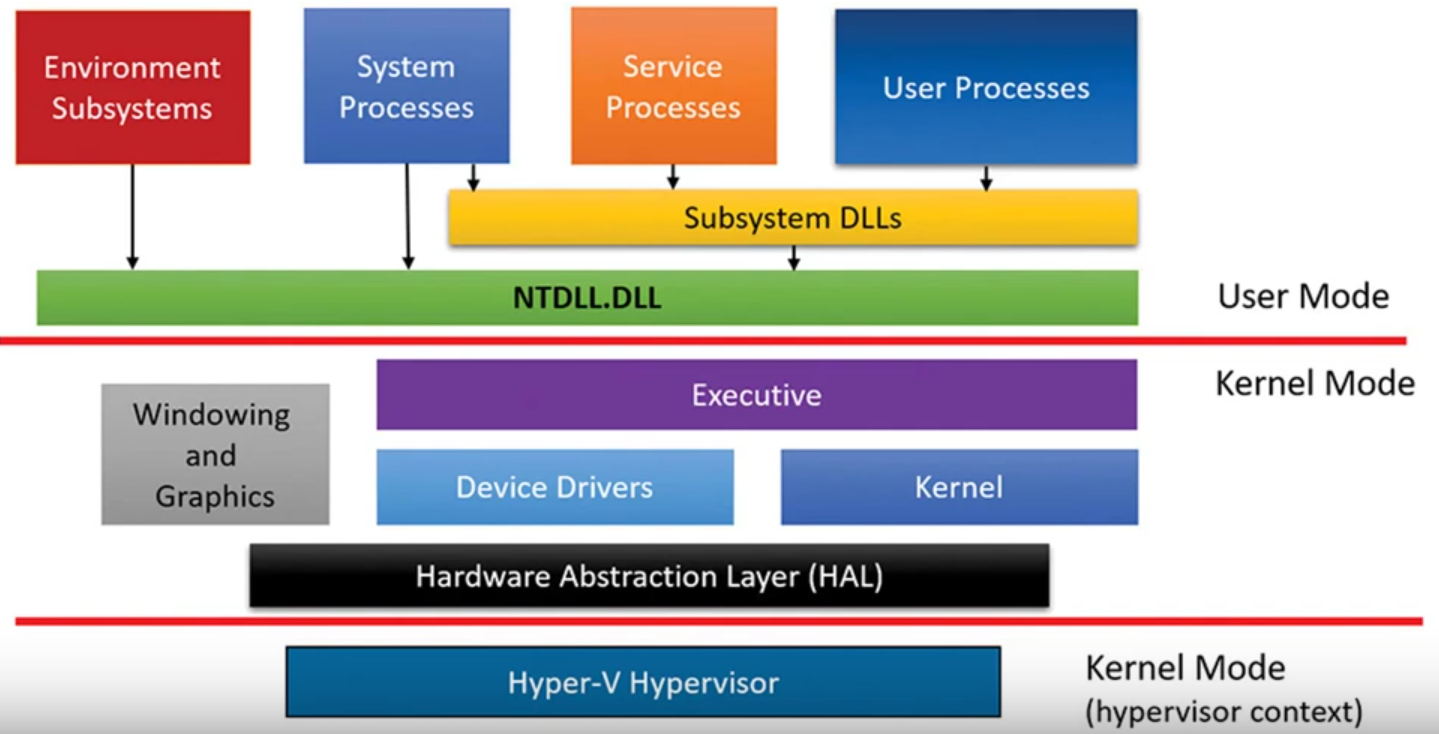
\includegraphics[width=\linewidth]{knowledge/internals/images/simplified-archi.png}
    \caption{Simplified archi}
    \label{fig:windows_siplified_archi}
\end{figure}

\begin{itemize}
    \item user-mode:
        \begin{itemize}
            \item {\bf Service processes} are processes that host Windows services, such as the Task Scheduler and Print Spooler services
            \item {\bf System processes} are fixed, or hardwired, processes, such as the logon process and the Session Manager, that are not Windows services. That is, they are not started by the {\bf Service Control Manager}
            \item Environment subsystem server processes implement part of the support for the OS environment, or personality, presented to the user and programmer. 
        \end{itemize}
    \item kernel-mode:
        \begin{itemize}
            \item {\bf Executive (\verb+Ntoskrnl.exe+)} contains the base OS services, such as memory management, process and thread management, security, I/O, networking, and inter-process communication.
            \item {\bf Windows kernel (\verb+Ntoskrnl.exe+)} consists of low-level OS functions, such as thread scheduling, interrupt and exception dispatching, and multiprocessor synchronization. It also provides a set of routines and basic objects that the rest of the executive uses to implement higher-level constructs.
            \item {\bf Device drivers} includes both hardware device drivers, which translate user I/O function calls into specific hardware device I/O requests, and non-hardware device drivers, such as file system and network drivers.
            \item {\bf Hardware Abstraction Layer (HAL)(\verb+hal.dll+)}  layer of code that isolates the kernel, the  device drivers, and the rest of the Windows executive from platform-specific hardware differences (such as differences between motherboards).
            \item {\bf windowing and graphics system (\verb+Win32k.sys+)} implements the graphical user interface (GUI) functions (aka Windows USER and GDI functions), such as dealing with windows, user interface controls, and drawing.
            \item {\bf hypervisor layer (\verb+hdvix64.exe+, \verb+hvax64.exe+)} is composed of a single component: the hypervisor itself. he hypervisor is itself composed of multiple internal layers and services, such as its own memory manager, virtual processor scheduler, interrupt and timer management, synchronization routines, \ldots.
        \end{itemize}
\end{itemize}


\verb+ntdll.dll+ : Internal support functions and system service dispatch stubs to executive functions

\verb+kernel32.dll, advapi32.dll, user32.dll,gdi32.dll+: core windows subsystem dlls
\section{Detailed system architecture}

\begin{figure}[!ht]
    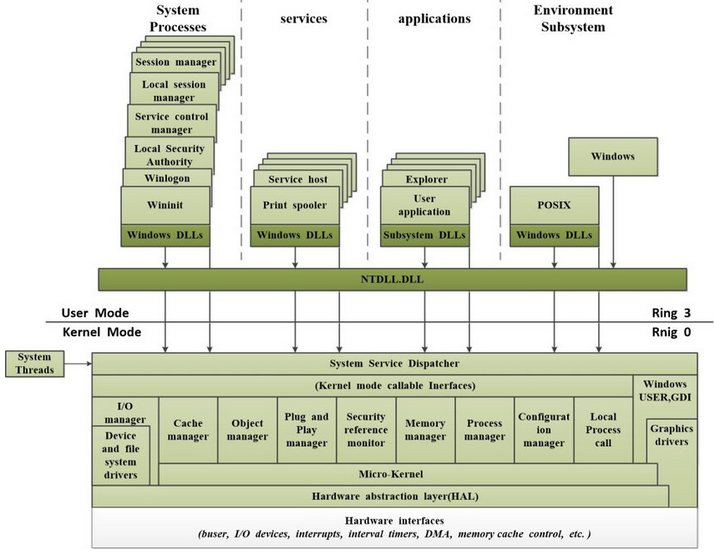
\includegraphics[width=\linewidth]{knowledge/internals/images/detailed-archi.png}
    \caption{Detailed archi}
    \label{fig:windows_detailed_archi}
\end{figure}


\subsection{Environment subsystems and subsystem DLLs}

\subsubsection{Introduction}
\begin{itemize}
    \item {\bf Environment subsystem} expose some subset of the base Windows executive system services to application programs. 
    \item Each subsystem can provide access to different subsets of the native services in Windows.
    \item Each executable image is bound to one and only one subsystem.
    \item When an image is run, the process creation code examines the subsystem type code in the image header so that it can notify the proper subsystem of the new process
    \item user applications don’t call Windows system services directly. Instead, they go through one or more subsystem DLLs.
    \item The {\bf environment subsystem processes}, running in user mode, are responsible for maintaining the state of the client applications running under their control.
\end{itemize}

When an application calls a function in a subsystem DLL, one of three things can occur:
\begin{itemize}
    \item The function is entirely implemented in user mode inside the subsystem DLL.
    \item The function requires one or more calls to the Windows executive.
    \item The function requires some work to be done in the environment subsystem process. In this case, a client/server request is made to the environment subsystem via an ALPC message sent to the subsystem to perform some operation. The subsystem DLL then waits for a reply before returning to the caller.
\end{itemize}

Some functions can be a combination of the second and third items just listed.

\subsubsection{Subsystem startup}
Subsystems are started by the Session Manager subsystem (SMSS) according to \verb+HKLM\SYSTEM\CurrentControlSet\Control\Session Manager\SubSystems+ 
\begin{itemize}
    \item \verb+Required+ value: list String that must be defined as registry value and define the list of the subsystems that load when the system boots
    \item \verb+Optional+ value: (load on demand) 
    \item \verb+kmode+: contains the file name of the kernel-mode portion of the Windows subsystem, \verb+Win32k.sys+
\end{itemize}

\subsubsection{Windows subsystem}

{\bf All subsystem rely on Windows subsystem to perform display I/O.}

The Windows subsystem consists of the following major components:
\begin{itemize}
    \item For each session, an instance of the \href{https://medium.com/@ijaz.faheem/windows-environment-subsystems-csrss-synch-with-windows-kernel-on-the-windows-user-process-164d57f2a81b}{CSRSS} loads four DLLs (\verb+Basesrv.dll+, \verb+Winsrv.dll+, \verb+Sxssrv.dll+, and \verb+Csrsrv.dll+) that contain support for the following:
        \begin{itemize}
            \item Various housekeeping tasks related to creating and deleting processes and threads
            \item Shutting down Windows applications
            \item Sending certain kernel notification messages to Windows applications as Window messages
            \item Side-by-Side (SxS)/Fusion and manifest cache support
            \item Several natural language support functions, to provide caching
        \end{itemize}
    \item A {\bf kernel-mode device driver} (Win32k.sys) that contains the following:
        \begin{itemize}
            \item The window manager (controls window displays; manages screen output; collects input
            from keyboard, mouse, and other devices; and passes user messages to applications)
            \item The Graphics Device Interface (GDI), which is a library of functions for graphics output devices
            \item Wrappers for DirectX
        \end{itemize}
    \item The {\bf console host process} (Conhost.exe), which provides support for console (character cell)
    applications
    \item The Desktop Window Manager
    \item Subsystem DLLs
    \item Graphics device drivers
\end{itemize}

{\bf CSRSS}:

Windows Kernel creates the process and thread and returns the handles to the method CreateProcessInternal (Kernelbase.dll). The CreateProcessInternal performs security operations (e.g., SxS) and constructs and sends a message to the Csrss process. The message contains information about process \& thread handles, section objects, flags, and other required information etc.

The Csrss is a critical system process, and it is responsible for managing the graphical user interface (GUI) on Windows systems. It also creates the process and keeps them in the organized process list. The process also monitors the user mode processes, and it can terminate a process if it crashes or because of any security issue.

The Csrss takes the process and thread handles and creates the duplicate process(\verb+CSR_Process+) and thread(\verb+CSR_Thread+) to monitor the process for Windows Subsystem.

The Csrss push the new process into the windows-subsystem wide process list(aka managed processes) on the successful creation of the Csrss process.


{\bf Win32k.sys}

The basic window-management requirements for Windows 10–based devices vary considerably depending on the device in question. For these reasons, the functionality of Win32K.sys has been split among  several kernel modules so that not all modules may be required on a specific system. This significantly reduces the attack surface of the window manager by reducing the complexity of the code and eliminating many of its legacy pieces.

Applications call the standard USER functions to create user-interface controls, such as windows and buttons, on the display. The window manager communicates these requests to the GDI, which passes them to the graphics device drivers, where they are formatted for the display device. A display driver is paired with a video miniport driver to complete video display support.

The GDI provides a set of standard two-dimensional functions that let applications communicate with graphics devices without knowing anything about the devices. GDI functions mediate between applications and graphics devices such as display drivers and printer drivers. The GDI interprets application requests for graphic output and sends the requests to graphics display drivers. It also provides a standard interface for applications to use varying graphics output devices. This interface enables application code to be independent of the hardware devices and their drivers. The GDI tailors its messages to the capabilities of the device, often dividing the request into manageable parts.

Because much of the subsystem—in particular, display I/O functionality—runs in kernel mode, only a few Windows functions result in sending a message to the Windows subsystem process: process and thread creation and termination and DOS device drive letter mapping (such as through subst.exe). In general, a running Windows application won’t cause many, if any, context switches to the Windows subsystem process, except as needed to draw the new mouse cursor position, handle keyboard input, and render the screen through CDD.

{\bf Console window host}

\verb+Conhost.exe+ process is spawned from the console-based process by the console driver (\verb+ConDrv.sys+) The process console-based process communicates with \verb+Conhost.exe+ using the console driver (\verb+ConDrv.sys+), by sending read, write, I/O control and other I/O request types.

Conhost.exe is designated as a server and the process using the console is the client.

\subsubsection{Other subsystem, Pico providers and WSL}


\subsection{Ntdll.dll}

\verb+Ntdll.dll+ is a special system support library primarily for the use of subsystem DLLs and images natives (not tied to a particular subsystem) applications.

It contains two types of functions:
\begin{itemize}
    \item {\bf System service dispatch stubs} to Windows executive system services. For each of these functions, \verb+Ntdll.dll+ contains an entry point with the same name. The code inside the function contains the architecture-specific instruction that causes a transition into kernel mode to invoke the {\bf system service dispatcher}. After verifying some parameters, this system service dispatcher calls the actual kernel-mode system service that contains the real code inside \verb+Ntoskrnl.exe+
    
    \item {\bf Internal support functions} used by subsystems, subsystem DLLs, and other native images such as:
        \begin{itemize}
            \item image loader (\verb+Ldr+ prefix), 
            \item heap manager, 
            \item Windows subsystem process communication functions (\verb+Csr+ prefix)
            \item general run-time library routines (\verb+Rtl+ prefix)
            \item support for user-mode debugging (\verb+DbgUi+ prefix)
            \item Event Tracing for Windows (\verb+Etw+ prefix)
            \item user-mode asynchronous procedure call (APC) dispatcher and exception dispatcher
            \item a small subset of the C Run-Time (CRT) routines, limited to those routines that are part of the string and standard libraries (\verb+memcpy+, \verb+strcpy+, \verb+sprintf+)
        \end{itemize} 

\end{itemize}

\subsection{Executive}

\subsubsection{Object manager}
The object manager responsible for creating, deleting, protecting, and tracking Windows executive objects and abstract data types that are used to represent OS resources such as processes, threads, and the various synchronization objects.



\subsection{system service dispatcher}

{\bf Part 2 chapter 8 page 91}

The kernel's trap handlers dispatch interrupts, exceptions and system service calls.

\subsection{Kernel}

\subsection{Hardware abstraction layer}
\subsection{Device drivers}
\subsection{System processes}
\section{Object manager}
{\bf Part 2 chapter 8}

The object manager responsible for creating, deleting, protecting, and tracking Windows executive objects and abstract data types that are used to represent OS resources such as processes, threads, and the various synchronization objects.
\begin{itemize}
    \item Sysinternals WinObj
    \item Process Explorer
    \item Sysinternals Handle
    \item Ressource Monitor
    \item Kernel debugger \verb+!handle+
\end{itemize}


\subsection{Object types}
three primary types of objects: 
\begin{itemize}
    \item executive objects: are objects implemented by various components of the executive
    \item kernel objects: not visible to user-mode code, provide fundamental capabilities such as synchronization on which executive objects are built (execuive objects encapsulate one or more kernel objects).
    \item GDI/ User objects: belong to windows subsystem and no not interact with kernel
\end{itemize}


\begin{itemize}
    \item the kernel maintains a list of all types of objects it supports.
    \item types have different supported operations and security properties
    \item \verb+Get-NtType+ 
\end{itemize}

\subsection{Object manager namespace (OMNS)}
\begin{verbatim}
    Get-ChildItem NtObject:\ | Sort-Object Name
    Get-ChildItem NtObject:\Dfs | Sort-Object Name
\end{verbatim}

The {\bf Primary Namespace} in Windows Object Manager refers to the main, global namespace that organizes system objects. It is essentially the root namespace where system objects are created and accessed. The primary namespace serves as the central reference point for all objects that can be accessed or manipulated in the system.

The objects in the primary namespace are globally accessible (subject to security and access control) and are referenced by their object names or handles.

Characteristics of the Primary Namespace:
\begin{itemize}
    \item Global Accessibility: Objects are available throughout the entire system.
    \item Well-Known Object Types: 
    \item Access Control: Access control mechanisms (like ACLs and security descriptors) are used to govern which processes can access objects in the primary namespace.
\end{itemize}

The {\bf Secondary Namespace} in the Windows Object Manager refers to a set of namespaces that are used for organizing objects in a more specific context or scope. hese namespaces are typically created for particular subsystems, applications, or kernel components that need to isolate or manage objects within their own boundaries.



Characteristics of the Secondary Namespace:
\begin{itemize}
    \item Specialized Scope: are usually specific to a particular subsystem or context, and they are isolated from the primary namespace
    \item Restricted Access: Objects might not be accessible by all processes. The access to secondary namespace objects can be more restricted, and processes might need to explicitly request access.
    \item Namespacing for Isolation: Secondary namespaces provide a way to logically isolate objects so that different applications or subsystems can have their own namespaces and avoid conflicts or unintended access to one another’s objects.
\end{itemize}


Examples of Secondary Namespace Objects:
\begin{itemize}
    \item Windows Registry:
    \item Security Objects: The Security namespace is another example, where security-related objects (like access tokens, privileges, and security descriptors) are organized and managed.
    \item Process Namespace: Each running process in Windows can have its own namespace for objects such as memory space, threads, and resources.
    \item Device Namespace
\end{itemize}

\subsection{Executive Objects}

Each Windows environment subsystem projects to its applications a different image of the operating
system. The executive objects and object services are primitives that the environment subsystems use
to construct their own versions of objects and other resources

Executive objects are typically created either by an environment subsystem on behalf of a user application or by variuous componets of the OS as part of their normal operation.

The Windows subsystem uses executive objects to export its own set of objects, many of which correspond directly to executive objects.


\subsection{Object structure}

\begin{itemize}
    \item The object manager controls the object headers and footer
    \item The executive components control the object body and type
\end{itemize}

\begin{figure}[!ht]
    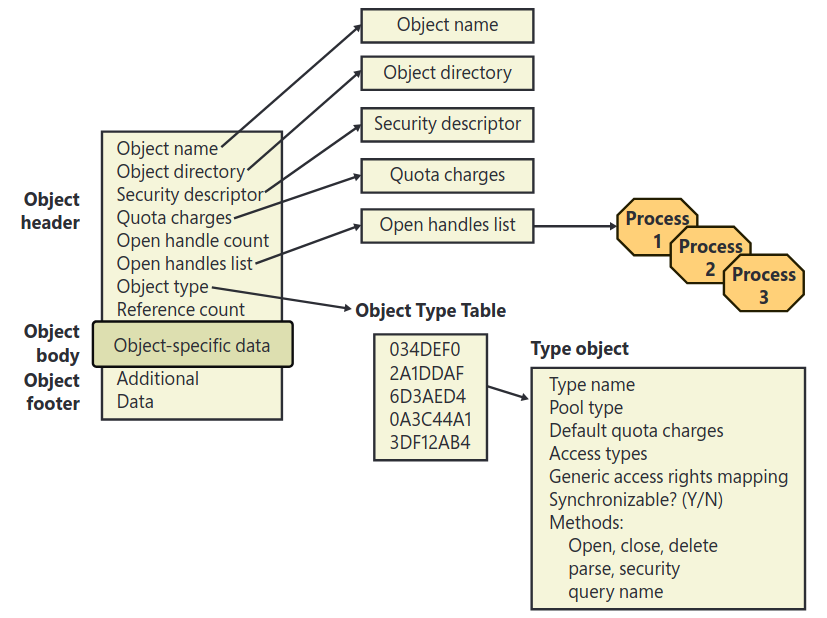
\includegraphics[width=\linewidth]{knowledge/internals/images/obj_structure.png}
    \caption{object structure}
    \label{fig:windows_object_structure}
\end{figure}

the object \verb+type object+ contains info common to each instance.

Additionally, up to eight optional subheaders exist: The name information header, the quota information header, the process information header, the handle information header, the audit information header, the padding information header, the extended information header, and the cre ator information header. 

If the extended information header is present, this means that the object has a footer, and the header will contain a pointer to it.

In addition to the object header, which contains information that applies to any kind of object, the subheaders contains optionalinformation regarding specific aspects ot he object. Note that these  structures are located at a variable offset from the start of the object header, the value of which depends on the number of subheaders associated with the main object header (except creator info).


{\bf windows internals part 2 chapter 8 page 131}

\subsection{Object methods}

{\bf windows internals part 2 chapter 8 page 140}

\subsubsection{Security method}
When an executive component defining an object doesn’t want to override the SRM’s default security policy, it marks the object type as having default security.


An object with default security (mutexes, events, semaphores) stores its security information in its header, and its security method is \verb+SeDefaultObjectMethod+

An object that doesn’t rely on default security must manage its own security information and supply a specific
security method.

A file object is an example of an object that overrides default security. The I/O manager, which defines the file object type, has the file system driver on which a file resides manage (or choose not to implement) the security for its files. Thus, when the system queries the security on a file object that represents a file on an NTFS volume, the I/O manager file object security method retrieves the file’s security using the NTFS file system driver

\subsection{Object handles and the process handle table}

{\bf windows internals part 2 chapter 8 page 143}

Each process object in the kernel has an {\bf handle table} containing:
\begin{itemize}
    \item the handle's numeric identifier
    \item the granted access to the handle
    \item the pointer to the object structure in kernel memory
\end{itemize}


\section{Security}

\subsection{Security system components}


\subsection{Object protection}
\begin{itemize}
    \item essence of discretionary access control and auditing
    \item Theoretically, anything managed by the executive object manager
    \item objects that are not exposed to user mode (such as driver objects) are usually not protected
    
\end{itemize}

To control who can manipulate an object, the security system must first be sure of each user’s identity.

When a process requests a handle to an object, the object manager and the security system use the  {\bf  caller’s security identification] and the {\bf object’s security descriptor} to determine whether the caller should be assigned a handle that grants the process access to the object it desires.

thread can assume a different security context than that of its process. This mechanism is called {\bf impersonation}.

It’s important to keep in mind that all the threads in a process share the same handle table, so when a
thread opens an object—even if it’s impersonating—all the threads of the process have access to the
object.

Sometimes, validating the identity of a user isn’t enough for the system to grant access to a resource that
should be accessible by the account. Windows achieves this kind of intra-user isolation with the {\bf Windows integrity mechanism}, which  implements integrity levels.

The Windows integrity mechanism is used by:
\begin{itemize}
    \item User Account Control (UAC)
    \item User Interface Privilege Isolation (UIPI)
    \item AppContainers
\end{itemize}




\subsubsection{Access checks}

thread must specify  up front, at the time that it opens an object, what types of actions it wants to perform on the object.

The object manager calls the SRM to perform access checks based on a thread’s desired access. If the access is granted, a handle is assigned to the thread’s process with which the thread (or other threads in the process) can perform further operations on the object.

Events causing the object manager to perform security access validation:
\begin{itemize}
    \item a thread opening an existin object using a name
    \item a process references an object using an existing handle
\end{itemize}

{\bf thread opening an existin object using a name}:
\begin{enumerate}
    \item Obj manager call \verb+ObpCreateHandle+ to create an entry in the process handle table that becomes associated with the object.
    \item \verb+ObpCreateHandle+ call \verb+ObpGrantAccess+ to see if the thread has permission to access the object
    \item \verb+ObpGrantAccess+ call \verb+ObCheckObjectAccess+ with the {\bf Security context} represented by an {\bf access token} the access type ({\bf access mask}) and a pointer to the object.
    \item \verb+ObCheckObjectAccess+ lock the object’s security descriptor and the security context of the thread (to prevent their modification)
    \item \verb+ObCheckObjectAccess+ then calls the object’s {\bf security method} to obtain the security settings of the object. 
    \item \verb+ObCheckObjectAccess+ then call \verb+SeAccessCheck+ from SRM with the object’s security information, the security identity of the thread and the access that the thread is requesting which return \verb+true+ or \verb+false+
    \item On success \verb+ObpCreateHandle+ calls the executive function \verb+ExCreateHandle+ to create the entry in the process handle table
\end{enumerate}


{\bf process references an object using an existing handle}:
The types of accesses the threads in the process are granted through the handle are stored with the handle by the object manager.

Some System services (for exemple NtWriteFile) uses the object manager function \verb+ObReferenceObjectByHandle+ to obtain a pointer to the file object from the handle


\verb+ObReferenceObjectByHandle+ accepts the access that the caller wants from the object as a parameter. After finding the handle entry in the process handle table, \verb+ObReferenceObjectByHandle+ compares the access being requested with the access granted for the thread.

The Windows security functions also enable Windows applications to define their own private objects and to call on the services of the SRM (through the \verb+AuthZ+ user-mode APIs) to enforce the Windows security model on those objects. Many kernel-mode functions that the object manager and other executive components use to protect their own objects are exported as Windows user-mode APIs. The user-mode equivalent of \verb+SeAccessCheck+ is the \verb+AuthZ API AccessCheck+. Windows applications can therefore leverage the flexibility of the security model and transparently integrate with the authentication and administrative interfaces that are present in Windows.

The essence of the SRM’s security model is an equation that takes three inputs: the security identity of a
thread, the access that the thread wants to an object, and the security settings of the object. The output is
either yes or no and indicates whether the security model grants the thread the access it desires. The
following sections describe the inputs in more detail and then document the model’s access-validation
algorithm.




\subsubsection{Access mask}
\href{https://learn.microsoft.com/en-us/windows/win32/secauthz/access-mask-format}{Access Mask Format}
\subsection{Tokens}

\subsubsection{Access token}
\subsubsection{Impersonation}
\subsubsection{Restricted tokens}

\section{Virtualization-based security}

\subsection{Architecture}

In Windows 10, Microsoft now leverages the Hyper-V hypervisor through the introduction of {\bf Virtual Trust Levels (VTLs)} to provide a new set of services known as {\bf virtualization-based security (VBS)} aka {\bf Virtual Secure Mode (VSM)}:
\begin{itemize}

    \item Device Guard: This provides Hypervisor Code Integrity (HVCI) for stronger code-signing guarantees over KMCS alone, and allows for the customization of the signature policy of the Windows OS, for both user-mode and kernel-mode code.
    \item Hyper Guard This protects key kernel-related and hypervisor-related data structures and code.
    \item Credential Guard This prevents unauthorized access to domain account credentials and secrets, combined with secure biometrics.
    \item Application Guard This provides an even stronger sandbox for the Microsoft Edge browser.
    \item Host Guardian and Shielded Fabric These leverage a virtual TPM (v-TPM) to protect a virtual machine from the infrastructure it’s running on
\end{itemize}


Virtual Trust Levels (VTLs).
\begin{itemize}
    \item operating system and its components are in a less privileged mode (\verb+VTL0+)
    \item VBS technologies run at \verb+VTL1+ (a higher privilege)
\end{itemize}

kernel and user mode exist within each VTL, and the hypervisor manages privileges across VTLs. The regular kernel and drivers, running in \verb+VTL0+, cannot be permitted to control and define \verb+VTL1+ resources.

\verb+VTL0+ is unaware of the existence of \verb+VTL1+.




\begin{figure}[!ht]
    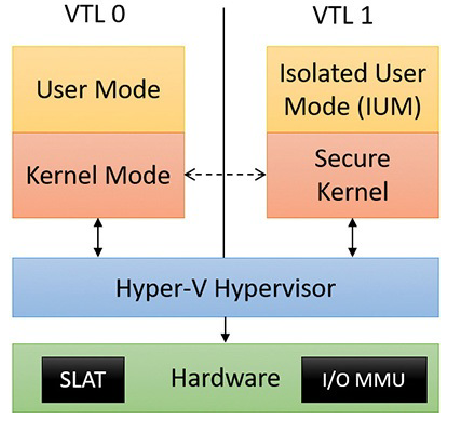
\includegraphics[width=\linewidth]{knowledge/internals/images/vbs-archi.png}
    \caption{VBS architecture}
    \label{fig:vbs_archi}
\end{figure}

\begin{figure}[!ht]
    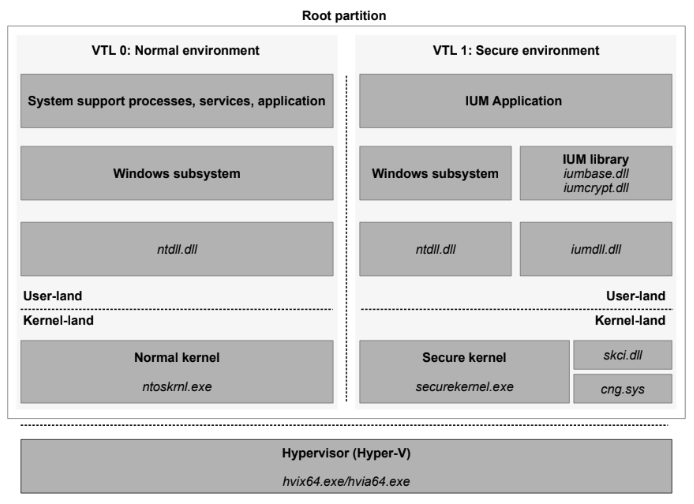
\includegraphics[width=\linewidth]{knowledge/internals/images/vbs-archi-detailed.png}
    \caption{VBS architecture detils}
    \label{fig:vbs_archi_detailed}
\end{figure}


with VBS:
\begin{itemize}
    \item \verb+VTL0+ kernel-mode code cannot touch \verb+VTL1+ user-mode  
    \item \verb+VTL1+ user-mode code cannot touch \verb+VTL0+ kernel-mode 
    \item \verb+\verb+VTL1++ user-mode applications must still go through regular Windows system calls and their respective access checks if they wish to access resources.
\end{itemize}

{\bf copy-on-write mechanisms, prevent \verb+VTL0+ applications from making changes to binaries used by \verb+VTL1+.}

The {\bf secure kernel (\verb+securekernel.exe+)} (aka {\emph proxy kernel}):
\begin{itemize}
    \item does not implement a full range of system capabilities, it hand-picks which system calls it will forward to the \verb+VTL0+ kernel. Any kind of I/O, including file, network, and registry-based, is completely prohibited. Graphics, as another example, are out of the question.
    \item have complete access to \verb+VTL0+ memory and resources
    \item limit the \verb+VTL0+ OS access to certain memory locations by leveraging CPU hardware support known as {\bf Second Level Address Translation (SLAT)}
    (SLAT).
\end{itemize} 

It can leverage:
\begin{itemize}
    \item {\bf Second Level Address Translation (SLAT)}:
        \begin{itemize}
            \item to limit the \verb+VTL0+ OS access to certain memory locations ({\bf Credential guard})
            \item nterdict and control execution of memory ({\bf Device Guard}) locations
        \end{itemize}
    \item {\bf I/O memory management unit (MMU)} which effectively virtualizes memory access for devices to prevent normal device drivers from leveraging hardware devices to directly access memory. This can be used to prevent device drivers from using direct memory access (DMA) to directly access the hypervisor or secure kernel’s physical regions of memory. This would bypass SLAT because no virtual memory is involved.
\end{itemize}

Because the hypervisor is the first system component to be launched by the boot loader, it can program the SLAT and I/O MMU as it sees fit, defining the \verb+VTL0+ and 1 execution environments. Then, while in \verb+VTL1+, the boot loader runs again, loading the secure kernel, which can configure the system further to its needs. Only then is the VTL dropped, which will see the execution of the normal kernel, now living in its \verb+VTL0+ jail, unable to escape.


Only a special class of specially {\bf signed binaries}, called {\bf Trustlets}, are allowed to execute in \verb+VTL1+. 
\begin{itemize}
    \item Each Trustlet has a unique identifier and signature
    \item the secure kernel has hard-coded knowledge of which Trustlets have been created so far
\end{itemize}

As such, it is impossible to create new Trustlets without access to the secure kernel and existing Trustlets cannot be patched in any way.

{\bf IUM}, it’s both:
\begin{itemize}
    \item an environment that restricts the allowed system calls that regular user-mode DLLs can make (thus limiting which of these DLLs can be loaded) 
    \item a framework that adds special secure system calls that can execute only under \verb+VTL1+. 
\end{itemize}    

These additional system calls are exposed in a similar way as regular system calls:
\begin{itemize}
    \item \verb+Iumdll.dll+: The IUM Native Layer DLL implements the secure system call stub. It’s the equivalent of \verb+Ntdll.dll+ of \verb+VTL0+.
    \item \verb+IumCrypt.dll+: Exposes public/private key encryption functions used for signing and integrity verification. Most of the crypto functions exposed to \verb+VTL1+ are implemented in \verb+Iumbase.dll+; only a small number of specialized encryption routines are implemented in \verb+IumCrypt+. \verb+LsaIso+ is the main consumer of the services exposed by \verb+IumCrypt+, which is not loaded in many other trustlets.
    \item \verb+Iumbase.dll+ The IUM Base Layer DLL is the library that implements most of the secure APIs that can be consumed exclusively by \verb+VTL1+ software. It provides various services to each secure process, like secure identification, communication, cryptography, and secure memory management. Trustlets do not usually call secure system calls directly, but they pass through \verb+Iumbase.dll+, which is the equivalent of \verb+kernelbase.dll+ in \verb+VTL0+.
\end{itemize}

A trustlet can be designed to run both in \verb+VTL1+ and \verb+VTL0+. In that case, it should only use routines implemented in the standard \verb+VTL0+ API surface since all the services available to \verb+VTL0+ are also implemented in \verb+VTL1+. For example, a trustlet can never do any registry I/O and any file I/O, but it can use synchronization routines, ALPC, thread APIs, and structured exception handling, and it can manage virtual memory and section objects. Almost all the services offered by the \verb+kernelbase+ and \verb+kernel32+ libraries perform system calls through \verb+Ntdll.dll+. In \verb+VTL1+, these kinds of system calls are {\emph translated} in normal calls and redirected to the \verb+VTL0+ kernel. Normal calls are often used by IUM functions and by the Secure Kernel itself. This explains why \verb+ntdll.dll+ is always mapped in every trustlet.



\subsection{Trustlet}




\subsection{Credential Guard}

Chapter 7

while RunAsPPL protection does guard the NT one-way function (NTOWF) and  TGT key from user-mode attackers, it does not protect against kernel attackers or user-mode attackers that
leverage vulnerabilities drivers.

Credential Guard solves this problem by using another process, \verb+Lsaiso.exe+, which runs as a Trustlet. This process therefore stores the user’s s secrets in its memory, not in \verb+Lsass+.

As \verb+VTL1+ does not have any drivers or access to I/O of hardware of any kind, Isolated LSA cannot directly communicate with the other servers (KDC,\ldots). This is still the responsibility of the Lsass process.

This seemingly results in a problem: the TGT and its key/NTOWF transiently pass through Lsass during authentication, and the TGT and its key are somehow available to Lsass for the generation of service tickets.

This leads to two questions: How does Lsass send and receive the secrets from isolated ISA, and how can we prevent an attacker from doing the same?

To answer the first question, recall that Chapter 3, “Processes and jobs,” described which services are available to Trustlets. One was the Advanced Local Procedure Call (ALPC), which the Secure Kernel supports by proxying the \verb+NtAlpc*+ calls to the Normal Kernel. Then, the Isolated User Mode nvironment implements support for the RPC runtime library (Rpcrt4.dll) over the ALPC protocol, which allows a VTL 0 and VTL 1 application to communicate using local RPC just like any other application and service.


To answer the first question, Although Lsass sits in the middle as a proxy would, it only
sees encrypted traffic between the KDC and isolated LSA, without the ability to understand its contents.

Isolated LSA establishes a {\bf local session key}, which only lives in \verb+VTL1+, and then uses a secure protocol to send this session key encrypted with yet another key (user NTLM ?), which only the KDC has.

The KDC can then respond with the TGT and its key after encrypting it with the isolated LSA session key. Therefore, Lsass sees an encrypted message to the KDC (which it can’t decrypt) and an encrypted message from the KDC (which it can’t decrypt).


Because disabling Credential Guard (which is ultimately nothing more than a registry setting) is trivial for an attacker, Secure Boot and UEFI can be leveraged to prevent a non-physically present administrator from disabling Credential Guard.



\href{https://learn.microsoft.com/fr-fr/windows/security/identity-protection/credential-guard/how-it-works}{Fonctionnement de Credential Guard}

\href{https://learn.microsoft.com/fr-fr/windows/security/identity-protection/credential-guard/considerations-known-issues}{Considérations et problèmes connus liés à l’utilisation de Credential Guard}


\href{https://learn.microsoft.com/fr-fr/windows/security/identity-protection/remote-credential-guard?tabs=intune}{Protection des informations d’identification à distance}
\begin{itemize}
    \item \href{https://github.com/wh0amitz/BypassCredGuard}{Credential Guard Bypass Via Patching Wdigest Memory}
    \item \href{https://itm4n.github.io/credential-guard-bypass/}{Revisiting a Credential Guard Bypass}
\end{itemize}


\section{Notes}

\begin{itemize}
    \item Windows API functions These are documented, callable subroutines in the Windows API.
    \item Native system services (or system calls) These are the undocumented, underlying services in the OS that are callable from user mode
    \item Kernel support functions (or routines) These are the subroutines inside the Windows OS that can be called only from kernel mode
\end{itemize}

\subsection{Virtual memory}

\begin{itemize}
    \item virtual memory is composed of 4kb pages (memory chunk)
    \item on 32-bits:
        \begin{itemize}
            \item lower half of this address space (addresses \verb+0x00000000+ through \verb+0x7FFFFFFF+) to processes (2GB)
            \item higher half of this address space (addresses \verb+0x80000000+ through \verb+0xFFFFFFFF+) to OS (2GB)
        \end{itemize}
\end{itemize}

\subsection{Kernel mode vs. user mode}

To protect user applications from accessing and/or modifying critical OS data, Windows uses two
processor access modes:
\begin{itemize}
    \item user mode
    \item kernel mode: mode of execution in a processor that grants access to all system memory and all CPU instructions
\end{itemize}

The architectures of the x86 and x64 processors define four privilege levels to protect system code and data from being overwritten by code of lesser privilege. Windows uses privilege level (ring) 0 for kernel mode and privilege level (ring) 3 for user mode.

Virtual memory Pages in system space can be accessed only from kernel mode, whereas all pages in the user address space are accessible from user mode and kernel mode

Windows doesn’t provide any protection for private read/write system memory being used by components running in kernel mode. 


\subsection{Terminal Services and multiple sessions}
The first session is considered the services session, or session zero, and contains system service hosting processes.

The first login session at the physical console of the machine is session one, and additional sessions can be created through the use of the remote desktop connection program (Mstsc.exe) or through the use of fast user switching


\subsection{Objects and handles}

\begin{itemize}
    \item a {\bf kernel object} is a single, run-time instance of a statically defined {\bf object type}
    \item {\bf object type} comprises a system-defined data type, functions that operate on instances of the data type, and a set of object attributes.
    \item internal structure of an object is opaque
    \item {\bf object manager} must be called o get data out of or put data into an object
    \item Not all data structures in the Windows OS are objects. Only data that needs to be shared, protected, named, or made visible to user-mode programs (via system services) is placed in objects
\end{itemize}
\section{Tools}

\subsection{NtObjectManager}

\href{https://github.com/googleprojectzero/sandbox-attacksurface-analysis-tools}{NtObjectManager} PowerShell module (backed by its supporting .NET managed library NtApiDotNet) is a godsend for Windows security researchers. From dealing with symbolic links, auditing RPC servers, playing tricks with the Object Manager, to just messing about with Windows, it has a myriad of applications. As one trying to improve their own auditing skills and understanding Windows internals, I am grateful for it. Right now I’ll admit that I am just touching the surface of the capability of the toolset. There are some advanced use cases that I have yet to get my head around. This post will be a step in the right direction. Before we jump into how to use NtObjectManager for RPC auditing, let’s take a short walk through the history of the RPC capabilities within NtApiDotNet.

\begin{verbatim}
    Get-ChildItem NtObject:\ | Sort-Object Name
    Get-ChildItem NtObject:\Dfs | Sort-Object Name
    Get-NtType

\end{verbatim}

\section{links}

\begin{itemize}
    \item \href{hhttps://www.google.fr/books/edition/Windows_Security_Internals/b_fNEAAAQBAJ?hl=fr&gbpv=1&dq=windows%20security%20internals&pg=PA25&printsec=frontcover}{Windows Security Internals}
\end{itemize}


\chapter{Process}
\label{knowledge:process}
\section{Notes}

\subsection{Get IAT from process}
\begin{verbatim}
    // Get the base address of the current module (EXE)
    HMODULE hModule = GetModuleHandle(NULL);
    // Get the address of the IMAGE_DOS_HEADER (the base of the PE file)
    PIMAGE_DOS_HEADER pDOSHeader = (PIMAGE_DOS_HEADER)hModule;

    // Get the address of the IMAGE_NT_HEADERS
    PIMAGE_NT_HEADERS pNTHeaders = (PIMAGE_NT_HEADERS)((BYTE*)hModule + pDOSHeader->e_lfanew);

    // Get the address of the IMAGE_IMPORT_DESCRIPTOR (the IAT)
    PIMAGE_IMPORT_DESCRIPTOR pImportDescriptor = (PIMAGE_IMPORT_DESCRIPTOR)(
        (BYTE*)hModule + pNTHeaders->OptionalHeader.DataDirectory[IMAGE_DIRECTORY_ENTRY_IMPORT].VirtualAddress
    );
\end{verbatim}


\subsection{Process Environment Block (PEB)}

\href{https://github.com/Faran-17/Windows-Internals/blob/main/Processes%20and%20Jobs/Processes/PEB%20-%20Part%201.md}{PEB - Part 1.md}

\subsubsection{Structure}
\verb+ntdll.lib+

\href{https://metehan-bulut.medium.com/understanding-the-process-environment-block-peb-for-malware-analysis-26315453793f}{PEB fields frequently used by malware developers}, along with brief descriptions of each:
\begin{itemize}
    \item 
    \item \verb+0x002+ \verb+BeingDebugged+, Anti-Debug
    \item \verb+0x068+ \verb+NtGlobalFlag+, Anti-Debug
    \item \verb+0x018+ \verb+ProcessHeap+, Anti-Debug
    \item \verb+0x00c+ \verb+Ldr+, API Hashing
    \item \verb+0x008+ \verb+ImageBaseAddress+, Process Hollowing
    \item \verb+0x010+ \verb+ProcessParameters+, UAC Bypass
\end{itemize}


\begin{verbatim}
typedef struct _LIST_ENTRY {
    struct _LIST_ENTRY *Flink;
    struct _LIST_ENTRY *Blink;
} LIST_ENTRY, *PLIST_ENTRY, PRLIST_ENTRY;
    
typedef struct _UNICODE_STRING {
    USHORT Length;
    USHORT MaximumLength;
    PWSTR  Buffer;
} UNICODE_STRING, *PUNICODE_STRING;
\end{verbatim}

When a process running, Windows OS will allocates a \href{http://undocumented.ntinternals.net/index.html?page=UserMode%2FUndocumented%20Functions%2FNT%20Objects%2FProcess%2FPEB.html}{Process Environment Block (PEB)} structure for the process. The PEB is created by the kernel and it basically contains fields that provide information such as loaded modules, process parameters, environment variables, and many more.

\href{http://undocumented.ntinternals.net/index.html?page=UserMode%2FUndocumented%20Functions%2FNT%20Objects%2FProcess%2FPEB.html}{PEB\_LDR\_DATA} structure that contains information of loaded (EXEs/DLLs) modules, including the doubly-linked list \verb+InMemoryOrderModuleList+ 

\begin{verbatim}
typedef struct _PEB_LDR_DATA {
    ULONG                   Length;
    BOOLEAN                 Initialized;
    PVOID                   SsHandle;
    LIST_ENTRY              InLoadOrderModuleList;
    LIST_ENTRY              InMemoryOrderModuleList;
    LIST_ENTRY              InInitializationOrderModuleList;
} PEB_LDR_DATA, *PPEB_LDR_DATA;
\end{verbatim}

\begin{itemize}
    \item \verb+Lenght+: Size of structure, used by ntdll.dll as structure version ID.
    \item \verb+Initialized+ If set, loader data section for current process is initialized.
    \item \verb+SsHandle+: unknown
    \item \verb+InLoadOrderModuleList+: doubly linked list containing pointers to \verb+LDR_MODULE+ structure for previous and next module in load order
    \item \verb+InMemoryOrderModuleList+: same as \verb+InLoadOrderModuleList+ but in memory placement order 
    \item \verb+InInitializationOrderModuleList+: same as \verb+InLoadOrderModuleList+ but in memory initialization order 
\end{itemize}


\verb+InMemoryOrderModuleList+ a doubly linked list containing pointers to \href{http://undocumented.ntinternals.net/index.html?page=UserMode%2FUndocumented%20Functions%2FNT%20Objects%2FProcess%2FPEB.html}{LDR\_MODULE} structure for previous and next module in memory placement order.

\begin{verbatim}
typedef struct _LIST_ENTRY {
    struct _LIST_ENTRY *Flink; // 4 or 8 bytes
    struct _LIST_ENTRY *Blink; // 4 or 8 bytes
} LIST_ENTRY, *PLIST_ENTRY, PRLIST_ENTRY;

typedef struct _UNICODE_STRING {
    USHORT Length;
    USHORT MaximumLength;
    PWSTR  Buffer;
} UNICODE_STRING, *PUNICODE_STRING;

typedef struct _LDR_MODULE {
    LIST_ENTRY              InLoadOrderModuleList;
    LIST_ENTRY              InMemoryOrderModuleList;
    LIST_ENTRY              InInitializationOrderModuleList;
    PVOID                   BaseAddress; // 4 or 8 bytes
    PVOID                   EntryPoint;  // 4 or 8 bytes
    ULONG                   SizeOfImage; // 4 bytes
    UNICODE_STRING          FullDllName;
    UNICODE_STRING          BaseDllName;
    ULONG                   Flags;
    SHORT                   LoadCount;
    SHORT                   TlsIndex;
    LIST_ENTRY              HashTableEntry;
    ULONG                   TimeDateStamp;
} LDR_MODULE, *PLDR_MODULE;
\end{verbatim}


\subsection{access using assembly}

\begin{verbatim}
    include <stdio.h>
    #include <Windows.h>
    
    int main() {
        PVOID peb;
    
        __asm {
            mov eax, fs:[0x30]
            mov peb, eax
        }
    
        printf("PEB Address: %p\n", peb);
        return 0;
    }
\end{verbatim}

\verb+fs+, resp. \verb+gs+ is a segment register used in 32-bit, resp. 64-bit, Windows to access memory. In this case, \verb+fs:[0x30]+, resp. \verb+gs:[0x60]+,  is the offset within the TEB that contains a pointer to the PEB.

see~\href{https://en.wikipedia.org/wiki/Win32_Thread_Information_Block}{Win32 Thread Information Block} for more \verb+gs/fs+

\subsubsection{PEB walk}

\href{https://fareedfauzi.github.io/2024/07/13/PEB-Walk.html}{PEB Walk}

\subsubsection{links}


\subsection{Thread Environment Block (TEB)}

PEB and its content can be accessed from the user mode. However, before accessing the PEB, we have to first access the Thread Environment Block (TEB), which serves as an information board like PEB, but for the thread this time.

As the program code is running in the thread, in other words, the “inner layer”, we have to access the process’s PEB, the “outer layer,” through the TEB. Hence, we can say that TEB is a gateway to reach PEB in our case as illustrated in Figure 2.

\subsection{Process and security}

\verb+PROCESS_ACCESS_TOKEN+

\begin{verbatim}
    BOOL GetTokenInformation(
        [in]            HANDLE                  TokenHandle,
        [in]            TOKEN_INFORMATION_CLASS TokenInformationClass,
        [out, optional] LPVOID                  TokenInformation,
        [in]            DWORD                   TokenInformationLength,
        [out]           PDWORD                  ReturnLength
      );
\end{verbatim}

\href{https://learn.microsoft.com/fr-fr/windows/win32/api/winnt/ne-winnt-token_information_class}{TokenInformationClass}

en gros on appel une premiere fois pour demander la taille necesaire puis on alloue le buffer et on appel une seconde fois avec le pointeur sur le buffer


\subsection{Protected Process Light (PPL)}
\section{links}

\begin{itemize}
    \item \href{https://sealkisnotklaes.fr/articles/technique-API-hashing}{PEB Parsing \& API Hashing}
\end{itemize}















\part{LSA}
\chapter{Knowledge}
\label{lsa:knowledge}
\section{Notes}
\subsection{Extracting Secrets from LSA }
\begin{itemize}
    \item \href{https://blog.syss.com/posts/powershell-lsa-parsing/}{Extracting Secrets from LSA by Use of PowerShell}
    \item  \href{https://github.com/cube0x0/MiniDump}{C\# implementation of mimikatz/pypykatz minidump functionality to get credentials from LSASS dumps.}
    \item \href{https://github.com/skelsec/minidump}{Python library to parse and read Microsoft minidump file format}
    \item \href{https://formats.kaitai.io/windows_minidump/}{Windows MiniDump: format specification }
    \item \href{https://ricardojoserf.github.io/nativedump/}{Dumping lsass using only NTAPIs by hand-crafting Minidump files}
\end{itemize}
\subsection{Usefull libs}
\begin{itemize}
    \item \href{https://learn.microsoft.com/fr-fr/windows/win32/api/tlhelp32/}{tlhelp32.h}
\end{itemize}

\subsection{Staying Under the Radar}

\begin{itemize}
    \item \href{https://crypt0ace.github.io/posts/Staying-under-the-Radar/}{Staying Under the Radar - Part 1 - PPID Spoofing and Blocking DLLs}
    \item \href{https://crypt0ace.github.io/posts/Staying-under-the-Radar-Part-3/}{Staying Under the Radar - Part 3 - Unhooking DLLs}
\end{itemize}

\subsection{Check sandboxing}

\begin{itemize}
    \item Call rare-enumated API 
    \begin{verbatim}
        if (VirtualAllocExNuma(GetCurrentProcess(), IntPtr.Zero, 0x1000, 0x3000, 0x4, 0) == IntPtr.Zero)
        {
            return;
        }
    \end{verbatim}
\end{itemize}



\subsection{Evade in-memory scan}

\begin{itemize}
    \item Sleep to evade in-memory scan + check if the emulator did not fast-forward through the sleep instruction
    \begin{verbatim}
        var rand = new Random();
        uint dream = (uint)rand.Next(10000, 20000);
        double delta = dream / 1000 - 0.5;
        DateTime before = DateTime.Now;
        Sleep(dream);
        if (DateTime.Now.Subtract(before).TotalSeconds < delta)
        {
            Console.WriteLine("Charles, get the rifle out. We're being fucked.");
            return;
        }
    \end{verbatim}
\end{itemize}
\section{links}

\begin{itemize}
    \item 
\end{itemize}
















\part{EDR / AV}
\chapter{Minidump}
\label{edr:misc}
\section{IAT unhook}

\subsection{links}
\begin{itemize}
    \item \href{https://alice.climent-pommeret.red/posts/how-and-why-to-unhook-the-import-address-table/}{EDR Bypass : How and Why to Unhook the Import Address Table}
    \item \href{https://securitymaven.medium.com/anatomy-of-iat-and-eat-hooking-9612eb15baf1}{Anatomy of IAT and EAT Hooking}
\end{itemize}
\section{Notes}


\subsection{API hashing}


\section{links}

\begin{itemize}
    \item 
\end{itemize}
















\part{EDR / AV}
\chapter{Minidump}
\label{edr:misc}
\section{IAT hooking}

\subsection{links}
\begin{itemize}
    \item \href{https://securitymaven.medium.com/anatomy-of-iat-and-eat-hooking-9612eb15baf1}{Anatomy of IAT and EAT Hooking}
    \item \href{https://github.com/m0n0ph1/IAT-Hooking-Revisited}{IAT Hooking Revisited}
\end{itemize}
\section{Notes}

\subsection{Reflective Loading of PE File}

\begin{itemize}
    \item \href{https://owl4444.github.io/2023/09/05/Relocation_Table_and_IAT_Fixing/}{Relocation Table and Import Address Table (IAT) in Reflectively Loaded PE File}
\end{itemize}
\section{links}

\begin{itemize}
    \item 
\end{itemize}
















\part{Links}
\chapter{Misc}
\label{links:misc}

\section{Code snippets}

\begin{itemize}
    \item \href{https://github.com/chvancooten/OSEP-Code-Snippets/tree/main}{chvancooten/OSEP-Code-Snippets}
\end{itemize}

















\end{document}
